\documentclass[11pt,a4paper,twocolumn]{article}
\usepackage[utf8]{inputenc}
\usepackage{amsmath}
\usepackage{graphicx}
\usepackage{hyperref}
\usepackage{setspace}
\usepackage{enumerate}
\usepackage{hyperref}
\hypersetup{
    colorlinks=true,
    linkcolor=blue,
    filecolor=magenta,      
    urlcolor=red,
}
\title{Assignment7}
\author{Aravind A Anil}
\date{\today}

\begin{document}
\maketitle
\begin{flushleft}
\textbf{Download the python codes from here:}
\fbox{\href{https://github.com/aravind11007/Probability--and--Random--Variable/blob/main/Assignment7/Assignment7.py}{pythoncode}}\\[5pt]
\textbf{Download all latex code from here:}
\\\fbox{\href{https://github.com/aravind11007/Probability--and--Random--Variable/blob/main/Assignment7/main.tex}{latex}}

\textbf{Problem statement:}A person plays a game of tossing a coin thrice.For each head,he is given Rs 2 by the organiser of the game and for each tail,he has to give Rs 1.50 to the organiser.Let X denotes the amount gained or lost by the person.show that X is random variable and exhibit it as a function on the sample space of the experiment\\
When three coins are tossed the possible outcomes are,\\
s=\{HHH,HHT,HTH,THH,TTH,THT,HTT,TTT\}\\
Let X:amount gained or lose\\
For each head,he wins Rs.2\\
\& for each tail he loses Rs.1.5\\
We have to calculate the values of X and have to check if the values are real values\\
\begin{table}[h!]
    \centering
    \begin{tabular}{|c|c|}
    \hline
         &X  \\[5pt]
         \hline
         X(HHH)&2+2+2=6\\[4pt]
         \hline
         X(HHT)&2+2-1.5=2.5\\[4pt]
         \hline
         X(HTH)&2-1.5+2=2.5\\[4pt]
         \hline
         X(THH)&-1.5+2+2=2.5\\[4pt]
         \hline
         X(TTH)&-1.5-1.5+2=-1\\[4pt]
         \hline
         X(THT)&-1.5+2-1.5=-1\\[4pt]
         \hline
         X(HTT)&2-1.5-1.5=-1\\[4pt]
         \hline
         X(TTT)&-1.5-1.5-1.5=-4.5\\
         \hline
    \end{tabular}
    \caption{\textbf{Possible values}}
\end{table}
\end{flushleft}
Here values of X can be 6,2.5,-1,-4.5\\
All these are real values\\
Hence,\textbf{X=\{6,2.5,-1,-4.5\}}\\
\& X is a \textbf{Random Variable}
\begin{table}[h!]
    \centering
    \begin{tabular}{|c|c|c|c|c|}
    \hline
         X&6&2.5&-1&-4.5  \\[5pt]
         \hline
         P(X)&$\frac{1}{8}$&$\frac{3}{8}$&$\frac{3}{8}$&$\frac{1}{8}$ \\[5pt]
         \hline
    \end{tabular}
    \caption{\textbf{Probability distribution(X)}}
    \label{tab:my_label}
\end{table}
\begin{figure}[h!]
    \centering
    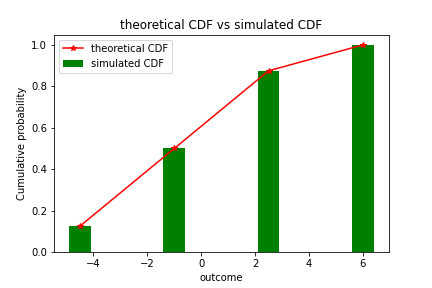
\includegraphics[width=10cm]{cdf.png}
    \caption{simulated CDF vs theoretical CDF}
\end{figure}
\begin{figure}[h!]
    \centering
    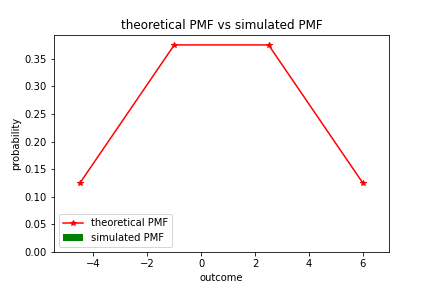
\includegraphics[width=10cm]{pmf.png}
    \caption{simulated PMF vs theoretical PMF}
\end{figure}
\end{document}
